\chapter{线性代数与微积分}

\section{线性映射的分析性质}

% 参考:《矩阵分析及其应用》张贤达
%      《矩阵分析》Horn
%      《泛函分析讲义》许全华
%      《数学分析讲义》于品

我们都熟知下面一点:$\mathcal{L}(\mathbf{R}^n, \mathbf{R}^m)$ 与 $\mathbf{R}^{m\times n}$ 同构,所以在某种意义上,我们研究线性映射与研究矩阵其实是一个效果. 线性映射其实只是线性空间之间的特别的函数,之前我们研究的东西一般多集中于线性映射的代数性质上,对于连续、有界等等更分析一些的性质我们并没有深入讨论. 本节我们将讨论线性映射的一些分析性质. 首先我们将从线性映射的范数切入:

\begin{definition}{线性映射的范数}{} \index{fanshu!xianxingyingshe@线性映射}
    对于线性映射 $A\in \mathcal{L}(\mathbf{R}^n, \mathbf{R}^m)$ 与 $x\in\mathbf{R}^n$,定义 $A$ 的\term{范数} $\Vert A \Vert$ 为 $\Vert A \Vert = \sup\limits_{\Vert x\Vert =  1} \Vert Ax\Vert$.
    % $\Vert A \Vert = \sup\limits_{\Vert x\Vert\leqslant 1} \Vert Ax\Vert$
\end{definition}

有些书籍称这样定义的范数为\term{诱导范数},大体是因为这种形式的定义不区分使用线性映射还是矩阵. 诱导范数反映出了线性映射伸张向量的能力,根据\[\Vert A\Vert = \sup\limits_{x\neq 0}\Vert A\frac{x}{\Vert x\Vert}\Vert = \sup\limits_{x\neq 0}\frac{\Vert Ax\Vert}{\Vert x\Vert},\]以及\[\Vert Ax\Vert = \Vert x\Vert \Vert A\frac{x}{\Vert x\Vert}\Vert \leqslant \Vert x\Vert \Vert A\Vert,\]这样就可以定义线性映射 $A$ 在 $x$ 方向的\term{伸张系数}$\dfrac{\Vert Ax\Vert}{\Vert x\Vert}$,并且 $\Vert A\Vert$ 的几何意义是一切方向的伸张系数的上确界.

注意到,对于一般的线性空间 $V$,如果范数定义得当,就算是 $V$ 是无穷维的,我们对有限维线性空间上的线性映射定义的范数施用在无穷维线性空间上的线性映射也是有意义的,但我们敏锐的嗅觉告诉我们,一旦加上了``无穷维''这个不容易处理的条件,无穷维线性空间上的线性映射的性质就会变得更加复杂,我们暂且不对其继续深入讨论.

诱导范数满足下面四条性质,读者可以简单验证:

\begin{theorem}{}{}
    设 $A\in \mathcal{L}(\mathbf{R}^n, \mathbf{R}^m),\enspace B\in \mathcal{L}(\mathbf{R}^l, \mathbf{R}^n)$,则
    \begin{enumerate}
        \item 正定性:$\Vert A\Vert\geqslant 0$,且 $\Vert A\Vert=0$ 当且仅当 $A=0$;
        \item 绝对齐次性:若$\lambda\in \mathbf{R}$,$\Vert \lambda A\Vert = \vert\lambda\vert \Vert A\Vert$;
        \item 次可加性:$\Vert A+B\Vert\leqslant\Vert A\Vert+\Vert B\Vert$;
        \item 次可乘性:$\Vert AB\Vert\leqslant\Vert A\Vert\Vert B\Vert$.
    \end{enumerate}
\end{theorem}

满足前三条性质的函数叫做\term{范数},若还满足第四条性质,就称其为\term{环范数}.

\begin{proof}
    \begin{enumerate}
        \item 显然;
        \item $\Vert \lambda A\Vert=\sup\limits_{\Vert x\Vert =  1}\Vert \lambda Ax\Vert = \vert\lambda\vert \sup\limits_{\Vert x\Vert = 1}\Vert Ax\Vert = \vert\lambda\vert \Vert A\Vert$;
        \item $\Vert A+B\Vert=\sup\limits_{\Vert x\Vert = 1}\Vert (A+B)x\Vert = \sup\limits_{\Vert x\Vert = 1}\Vert Ax + Bx\Vert\leqslant\sup\limits_{\Vert x\Vert = 1}\Vert Ax\Vert+\sup\limits_{\Vert x\Vert = 1}\Vert Bx\Vert=\Vert A\Vert+\Vert B\Vert$;
        \item $\Vert AB\Vert=\sup\limits_{\Vert x\Vert = 1}\Vert ABx\Vert=\sup\limits_{\Vert x\Vert = 1}\Vert A(Bx)\Vert\leqslant\sup\limits_{\Vert x\Vert = 1}\Vert A\Vert\Vert Bx\Vert\leqslant\Vert A\Vert\sup\limits_{\Vert x\Vert = 1}\Vert Bx\Vert=\Vert A\Vert\Vert B\Vert$.
    \end{enumerate}
\end{proof}

按我们诱导范数的定义,很容易证明任一矩阵的范数肯定大于其任何一个特征值的绝对值. 对于任何形式定义的范数,这个陈述也一样成立,证明并不困难,我们将其留作习题.

% 参考:https://math.stackexchange.com/questions/2855044/why-is-the-norm-of-a-matrix-larger-than-its-eigenvalue

将向量的内积加以推广,我们还可以定义矩阵的内积与另一种范数:

\begin{definition}{矩阵的内积}{} \index{neiji!juzhen@矩阵}
    对于 $\mathbf{F}^{m\times n}$ 上的矩阵 $A$ 与 $B$,$A = \left[\vec{a_1}, \vec{a_2}, \ldots, \vec{a_n}\right]$ 与 $B = \left[\vec{b_1}, \vec{b_2}, \ldots, \vec{b_n}\right]$,将其写成列向量拼接的形式:定义矩阵 $A$ 的\term{列向量化}为$mn \times 1$ 向量 \[\vec{a} = \operatorname{vec}(A) = \begin{pmatrix} \vec{a_1} \\ \vec{a_2} \\ \vdots \\ \vec{a_n} \end{pmatrix},\]
    借此定义矩阵 $A$ 与 $B$ 的内积为 $\langle A, B\rangle \colon \mathbf{F}^{m\times n}\times\mathbf{F}^{m\times n}\to\mathbf{F}$,\[\langle A, B\rangle = \langle \operatorname{vec}(A), \operatorname{vec}(B)\rangle.\]
    常见形式为 Frobenius 内积 \[\langle A, B\rangle = \tr(A^{T}B) = \sum_{i=1}^{m}\sum_{j=1}^{n}a_{ij}b_{ij}.\]
\end{definition}

这样定义的内积高度依赖于我们向量内积的选取,并且仅对于矩阵有意义. 借助这种矩阵向量化的思想,我们可以定义矩阵的\term{``元素形式''范数}:

\begin{definition}{``元素形式''范数}{}
    对于矩阵 $M\in \mathbf{F}^{m\times n}$ 定义 $M$ 的\term{``元素形式''范数}为下面的 $\ell_p$ 矩阵范数 \[\Vert M\Vert_p = \lVert \operatorname{vec}(M) \rVert _p = \left(\sum_{i = 1}^{m}\sum_{j = 1}^{n} \vert a_{ij}\vert^p\right)^{1/p}.\]
    很容易可以验证其满足范数的三条性质,当 $p$ 不取到 $+\infty$ 时,该范数同时也是环范数,当 $p = 2$ 时,称该范数为 Frobenius 范数.
\end{definition}

这样一来,我们成功将线性映射组成的线性空间成功``升格''成了赋范线性空间,之后甚至可以在其之上继续研究,这就形成了泛函分析中丰富的算子理论,但与本节相隔甚远,仅介绍一些较为基础的内容. 恰如我们在实数域等赋范空间上定义了多种范数一样,在线性映射组成的线性空间中,我们可以根据需求的不同使用不同的范数进行研究,但是重要的是知道不同范数之间可能存在的关系. 幸运的是,在有限维赋范线性空间上,不同范数之间是等价的,让我们一步一步来看:

赋范线性空间 $(X, \Vert \cdot \Vert)$ 当然是度量空间,对于 $x, y\in X$,只需要定义 $d(x, y) = \Vert x-y\Vert$ 就可以轻易诱导出一个度量,而连续与收敛的概念恰恰就定义在度量空间上,不妨回忆一下先:

\begin{definition}{收敛}{}
    设 $V$ 是一个实的或者复的赋范空间,其范数为 $\Vert \cdot \Vert$,此范数诱导出的度量为 $d(x, y) = \Vert x - y\Vert$,称 $V$ 中的一个序列 $\left\{x^{(i)}\right\}$ \term{收敛}到 $x\in V$,当且仅当 \[\lim_{i\to\infty}d(x^{(i)} - x) = 0.\]
\end{definition}

\begin{definition}{连续}{}
    假设 $(X,d_X)$ 和 $(Y, d_Y)$ 是两个度量空间,$f\colon X\to Y$ 是这两个度量空间的映射. 假设 $x_0\in X$,$y_0 = f(x_0)\in Y$. 如果对于任意的 $\varepsilon>0$,都存在 $\delta>0$ 使得对于任意满足 $d_X(x, x_0) < \delta$ 的 $x\in X$,都有 $d_Y(f(x), y_0) < \varepsilon$,那么称 $f$ 在 $x_0$ 处\term{连续}. 如果 $f$ 在 $X$ 的每一点都连续,那么称 $f$ 是\term{连续映射}.
\end{definition}

在 $C[0, 1]$ 上,倘若我们定义了一系列范数,比如 $\ell_p$ 范数,可以举出例子表明同一序列在不同范数下可能收敛到不同的极限,我们在习题中将涉及到这一点. 但是在有限维赋范线性空间上,这样的奇怪现象并不会出现,这个的理论基础是下面的 Weierstrass 定理:

\begin{theorem}{Weierstrass 定理}{}
    设 $S$ 为一个具有给定范数 $\Vert \cdot \Vert$ 的有限维实线性空间 $V$ 的一个紧子集,设 $f\colon S\to\mathbf{R}$ 是一个连续函数,那么 $f$ 在 $S$ 上可以取得最大值与最小值,这就是说,存在两个点 $x_1, x_2\in S$ 使得对于任意 $x\in S$ 都有 \[f(x_1)\leqslant f(x)\leqslant f(x_2).\]
\end{theorem}

对应的拓扑基础知识可以参考很多拓扑学或分析学的教材,这里不再赘述.

\begin{lemma}{}{}
    设 $\Vert \cdot\Vert$ 是定义在实赋范向量空间 $V$ 上的一个范数,$m\geqslant 1$ 是一个给定的正整数,$x^{(1)}, x^{(2)}, \ldots, x^{(m)}\in V$ 是给定的向量组,又对任意的 $z = (z_1, \ldots, z_m)^\mathrm{T} \in \mathbf{R}^m$,可以定义 $x(z) = \sum\limits_{i=1}^{m}z_ix^{(i)}$,那么由 $x(z)$ 定义的函数 $g\colon \mathbf{R}^m\to \mathbf{R}$,
    \[g(z) = \Vert x(z)\Vert = \left\lVert \sum_{i=1}^{m}z_ix^{(i)}\right\rVert\] 是关于 Euclid 范数 $\Vert\cdot\Vert_2$ 一致连续的函数.
\end{lemma}

\begin{proof}
    设 $u = (u_1, \ldots, u_m)^\mathrm{T}$,$v = (v_1, \ldots, v_m)^\mathrm{T}$,那么
    \begin{align}
        \vert g(x(u)) - g(x(v))\vert
         & = \lvert \Vert x(u) \Vert - \Vert x(v) \Vert \rvert \leqslant \lVert x(u) - x(v)\rVert                                                           \\
         & = \left\lVert \sum_{i = 1}^{m} (u_i - v_i)x^{(i)}\right\rVert \leqslant \sum_{i = 1}^{m}\vert u_i - v_i\vert \Vert x^{(i)}\Vert                  \\
         & \leqslant \left(\sum_{i = 1}^{m}\vert u_i - v_i\vert^2\right)^{1/2}\left(\sum_{i = 1}^{m}\Vert x^{(i)}\Vert^2\right)^{1/2} =C\Vert u - v\Vert_2.
    \end{align}
    这个常数 $C = \left(\sum\limits_{i = 1}^{m}\Vert x^{(i)}\Vert^2\right)^{1/2}$ 仅仅与范数 $\Vert\cdot\Vert$ 以及给定的向量组 $x^{(1)}, x^{(2)}, \ldots, x^{(m)}$ 有关,一定满足 $0 \leqslant C<\infty$,所以 $g$ 一定是一致连续的.
\end{proof}

上面引理中要求赋范线性空间 $V$ 不一定是有限维的,但是对于下面这个关键刻画,有限维这个条件就是不可缺少的:

\begin{theorem}{}{}
    设 $f_1$ 和 $f_2$ 是有限维实向量空间 $V$ 上的一个实值函数,设 $\mathcal{B} = \left\{x^{(1)}, x^{(2)}, \ldots, x^{(m)}\right\}$ 是 $V$ 的一组基,对 $z = (z_1, z_2, \ldots, z_m)^\mathrm{T}\in \mathbf{R}^m$,定义 $x(z) = \sum\limits_{i=1}^{m}z_ix^{(i)}$. 若 $f_1$ 和 $f_2$ 为
    \begin{enumerate}
        \item 正的:对所有的 $x\in V$ 都有 $f_i(x)\geqslant 0$,且 $f_i(x) = 0$ 当且仅当 $x = 0$;
        \item 齐次的:对所有的 $x\in V$ 和所有的 $\lambda\in\mathbf{R}$ 都有 $f_i(\lambda x) = \Vert \lambda\Vert f_i(x)$;
        \item 连续的:$f_i$ 在 $V$ 上关于 Euclid 范数 $\Vert\cdot\Vert_2$ 是连续的,或者说 $f_i(x(z))$ 在 $\mathbf{R}^m$ 上关于 Euclid 范数是连续的.
    \end{enumerate}
    那么就存在正常数 $C_m$ 和 $C_M$ 使得对于所有 $x\in V$ 都有 \[C_mf_1(x) \leqslant f_2(x) \leqslant C_Mf_1(x).\]
\end{theorem}

满足正性、齐次性与连续性的有限维实向量空间上的实值函数被称为\term{预范数}\footnote{这里借用的是 Roger Horn 的《矩阵分析》中的用词,英文原文为 pre-norm,这里为了与 quasinorm 与 paranorm 作区分,故翻译为预范数.},最经典的预范数当然是范数,上面这个定理告诉我们:在有限维实赋范线性空间上,所有的预范数都相差有限倍. 下面我们证明一下这个定理:

\begin{proof}
    在单位球面 $S = \{z\in \mathbf{R}^m \mid \Vert z\Vert_2 = 1\}$ 上定义 $h(z) = \dfrac{f_2(x(z))}{f_1(x(z))}$,$S$ 是 $\mathbf{R}^m$ 上关于 Euclid 范数的紧子集,正定性和连续性保证了 $h(z)$ 在 $S$ 上也是连续的,带有 Euclid 范数的 $\mathbf{R}^m$ 上的 Weierstrass 定理保证了 $h$ 在 $S$ 上可以取到有限的正最大值 $C_M$ 和正的最小值 $C_m$,所以对所有的 $z\in S$ 都有 \[C_m\leqslant h(z) = \frac{f_2(x(z))}{f_1(x(z))}\leqslant C_M.\]
    因为对每个非零的 $z\in\mathbf{R}^m$ 都有 $z/\Vert z\Vert_2\in S$,根据其次性得知 \[f_i\left(x\left(\frac{z}{\Vert z\Vert_2}\right)\right) = f_i\left(\frac{1}{\Vert z\Vert_2}x(z)\right) = \frac{1}{\Vert z\Vert_2}f_i(x(z)),\]
    所以对于所有非零的 $z\in\mathbf{R}^m$ 都有 \[C_m f_1(x(z))\leqslant f_2(x(z))\leqslant C_M f_1(x(z)).\]
    该式对 $z = 0$ 也成立,因为 $f_1(0) = f_2(0) = 0$,每一个 $v\in V$ 都可以表示成 $\mathcal{B}$ 的线性组合的形式,所以自然可以表示成 $v = x(z)$ 的形式,这样结论中的不等式对所有的 $x\in V$ 都成立.
\end{proof}

证明的核心是在 $S$ 上应用 Weierstrass 定理,这要求 $S$ 一定是紧的,但是 $S$ 的紧性仅在有限维空间中是有保证的,所以这个定理也只适用于有限维空间.

既然有限维线性空间上的范数都差不多,那么我们可以完全解决上面的问题:在有限维实赋范线性空间上,无论我们使用哪种范数,我们都可以得到相同的收敛性质. 也就是:

\begin{corollary}{}{}
    设 $\Vert \cdot\Vert_\alpha$ 和 $\Vert \cdot\Vert_\beta$ 是定义在有限维实赋范向量空间 $V$ 上的两个范数,又如果存在 $\left\{x^{(i)}\right\}$ 是 $V$ 中一列给定的向量,$x\in V$ 是给定的向量,那么关于 $\Vert \cdot\Vert_\alpha$ 有 $\left\{x^{(i)}\right\}$ 收敛到 $x$ 当且仅当关于 $\Vert \cdot\Vert_\beta$ 有 $\left\{x^{(i)}\right\}$ 收敛到 $x$.
\end{corollary}

证明非常简单,直接略过则可. 在实向量空间上,如果两个范数关于同一列向量序列的收敛性是等价的,那么这两个范数是\term{等价}的. 上面的论述告诉我们:\textbf{有限维实线性空间上的范数都是等价的},这就是我们在有限维赋范线性空间上研究范数的一个重要结论. 无限维线性空间上的结论就要复杂一些,一个比较简单的结果是:无限维线性空间上总存在两个不等价的范数,读者可以阅读有关矩阵分析的书籍来了解更多.

线性映射终归也是一个``线性的函数'',所以自然可以考虑它的有界性和连续性,这里就需要利用范数来进行研究了:

\begin{definition}{赋范线性空间上的有界映射}{}
    设 $A$ 是赋范线性空间 $X$ 到赋范线性空间 $Y$ 的线性映射,如果存在常数 $M\geqslant 0$ 使得对于任意 $x\in X$,都有 \[\Vert Ax\Vert\leqslant M\Vert x\Vert,\]
    那么称 $A$ 是\term{有界映射}.
\end{definition}

\begin{theorem}{}{}
    对于线性赋范空间 $X$ 和 $Y$,从$X$ 到 $Y$ 的线性映射 $A$ 是有界映射的充分必要条件是 $A$ 将所有有界集映射为有界集.
\end{theorem}

\begin{proof}
    设 $A$ 将所有有界集映射为有界集,那么 $A$ 将单位球面 $S=\{x\in X \mid \Vert x\Vert=1\}$ 映射为一个有界集,那么存在常数 $M\leqslant 0$ 使得对于 $y\in S$ 有 $\Vert Ay\Vert\leqslant M$,当 $x = 0$ 的时候,$\Vert Ax\Vert \leqslant M\Vert x\Vert$自然成立,当 $x \neq 0$ 的时候,取 $y=\dfrac{x}{\Vert x\Vert}$,那么 \[\frac{\Vert Ax\Vert}{\Vert x\Vert} = \left\Vert A\frac{x}{\Vert x\Vert}\right\Vert = \Vert Ay\Vert \leqslant M.\] 这就说明了 $A$ 为有界映射.

    反过来,如果 $A$ 是有界映射,设 $B$ 是 $X$ 中的有界集,那么存在常数 $N$ 使得对于任意 $x\in B$ 都有 $\Vert x\Vert\leqslant N$,那么对于任意 $x\in B$,有 \[\Vert Ax\Vert\leqslant M\Vert x\Vert\leqslant MN,\]这就说明了 $A$ 将有界集映射为有界集.
\end{proof}

值得注意的是,利用 Zorn 引理可以证明:任何无限维赋范线性空间上必存在定义在全空间上的无界线性算子。

\begin{theorem}{赋范线性空间上的连续映射}{}
    设 $A$ 是赋范线性空间 $X$ 到赋范线性空间 $Y$ 上的线性映射,假设 $A$ 在某一点 $x_0\in X$ 处连续,那么 $A$ 是 $X$ 上的连续映射.
\end{theorem}

这体现了线性算子和一般的函数之间的显著差异:线性性能够将一个局部的性质放大到整体的性质,这是这个证明的精髓。

\begin{proof}
    对任意一点 $x\in X$,设 $\{x_n\}$ 是 $X$ 中的一个序列,满足 $\lim\limits_{n\to\infty}x_n = x$,那么 $\lim\limits_{n\to\infty}x_n - x + x_0 = x_0$,由假设 $A$ 在 $x_0$ 处连续,所以 \[\lim\limits_{n\to\infty}A(x_n - x + x_0) = A(x_0),\]
    所以 \[\lim\limits_{n\to\infty}Ax_n = Ax.\]
    这就说明了 $A$ 在 $x$ 处连续. 由 $x$ 的任意性可知 $A$ 在 $X$ 上是连续映射.
\end{proof}

下面这个定理给出了线性映射的有界性与连续性之间的关系:

\begin{theorem}{有界线性变换定理}{}
    从赋范线性空间 $X$ 到赋范线性空间 $Y$ 上的线性映射 $A$ 是有界映射的充分必要条件是 $A$ 是连续映射.
\end{theorem}

更进一步的,如果 $A\in \mathcal{L}(\mathbf{R}^n, \mathbf{R}^m)$ 那么可以直接得到 $A$ 是有界且一致连续的. 当我们取 $\mathbf{R}^n$ 上的一组标准基 $\{e_1, e_2, \ldots, e_n\}$,设 $x\in \mathbf{R}^n$,$\Vert x\Vert \leqslant 1$,那么 $x$ 就可以表示为 $x = \displaystyle\sum_{i=1}^{n} x_ie_i$,$\vert x_i \vert \leqslant 1$. 于是
\[\Vert Ax\Vert = \left\Vert \sum_{i=1}^{n} x_iAe_i\right\Vert \leqslant \sum_{i=1}^{n}\vert x_i\vert \Vert Ae_i\Vert \leqslant \sum_{i=1}^{n}\Vert Ae_i\Vert.\]
所以\[\Vert A\Vert \leqslant \sum_{i=1}^{n}\Vert Ae_i\Vert < \infty.\]
并且因为当 $x, y\in \mathbf{R}^n$ 时,$\Vert Ax - Ay \Vert \leqslant \Vert A\Vert\Vert x-y\Vert$,所以 $A$ 是一致连续的.

\begin{theorem}{}{}
    设 $\Omega$ 为 $\mathbf{R}^n$ 上所有可逆线性算子的集合.
    \begin{enumerate}
        \item 若 $A\in \Omega$,$B\in \mathcal{L}(\mathbf{R}^n)$,并且 \[\Vert B-A\Vert\cdot\Vert A^{-1}\Vert < 1,\]那么 $B\in \Omega$;
        \item $\Omega$ 是 $\mathcal{L}(\mathbf{R}^n)$ 的开集,映射 $A\to A^{-1}$ 是 $\Omega$ 上的连续映射.
    \end{enumerate}
\end{theorem}

\begin{proof}
    \begin{enumerate}
        \item 令 $\Vert A^{-1}\Vert = \dfrac{1}{\alpha}$,$\Vert B-A\Vert = \beta$,那么 $\beta < \alpha$,对于每一个 $x\in \mathbf{R}^n$,
              \begin{align}
                  \alpha\Vert x\Vert & = \alpha\Vert A^{-1}Ax\Vert \leqslant \alpha \Vert A^{-1}\Vert \cdot \Vert Ax \Vert                        \\
                                     & = \Vert Ax\Vert \leqslant \Vert (A - B)x\Vert + \Vert Bx\Vert \leqslant \beta\Vert x\Vert + \Vert Bx\Vert,
              \end{align}
              因此 \[(\alpha - \beta)\Vert x\Vert \leqslant \Vert Bx\Vert,\enspace \forall x\in \mathbf{R}^n.\]
              因为 $\alpha - \beta > 0$,所以只要 $x\neq 0$,就有 $Bx\neq 0$,所以 $B$ 就是一一映射,也一定是可逆映射. 这对所有满足 $\Vert B - A\Vert < \alpha$ 的 $B$ 都成立,这就完成了证明并且证明了 $\Omega$ 是开集;
        \item 在 $(\alpha - \beta)\Vert x\vert \leqslant \Vert Bx\Vert$ 将 $x$ 换成 $B^{-1}y$ 可以得到 \[(\alpha - \beta)\Vert B^{-1}y\vert \leqslant \Vert BB^{-1}y\Vert = \Vert y\Vert,\enspace y\in \mathbf{R}^n,\]
              这说明 $\Vert B^{-1}\Vert \leqslant \dfrac{1}{\alpha - \beta}$,于是根据恒等式 $B^{-1} - A^{-1} = B^{-1}(A - B)A^{-1}$ 与 $\Vert AB\Vert \leqslant \Vert A\Vert \Vert B\Vert$ 可以得到 \[\Vert B^{-1} - A^{-1}\Vert \leqslant \Vert B^{-1}\Vert\Vert A - B\Vert\Vert A^{-1}\Vert \leqslant \dfrac{\beta}{\alpha(\alpha - \beta)}.\]
              当 $B\to A$ 时,$\beta\to 0$,这就证明了 $A\to A^{-1}$ 是连续映射.
    \end{enumerate}
\end{proof}

在做题的时候,我们经常会遇见可逆矩阵,这不是因为我们的题目有多么``好心'',而是因为可逆矩阵``在数量上''是远远多于不可逆矩阵的. 事实上有:实数域上的不可逆矩阵在 $\mathbf{R}^{n\times n}$ 中为零测集,可逆矩阵在 $\mathbf{R}^{n\times n}$ 中是稠密的,每个不可逆矩阵都可以被一列可逆矩阵逼近.

前半段很简单,若 $A$ 为不可逆矩阵,那么 $\det A = 0$,取出 $A$ 的每个元素 $a_i \enspace(1\leqslant i\leqslant n^2)$,将 $a_i$ 视为 $\mathbf{R}$ 上的一个变量,那么 $\det A$ 关于每个分量 $a_i$ 就是一个多项式,这个多项式的零点对应的元素形成的矩阵构成的集合就是不可逆矩阵的集合,这个集合构成一个``薄薄的''超曲面,因此是零测的.
对于后半段,我们证明这样的结论:$A\in\mathbf{R}^{n\times n}$ 为任意取的一个矩阵,则在任意范数下都存在着可逆矩阵任意趋近 $A$,这就说明了可逆矩阵在 $\mathbf{R}^{n\times n}$ 中是稠密的. 另取任意可逆矩阵 $B\in\mathbf{R}^{n\times n}$,构造关于 $t\in \mathbf{R}$ 的多项式函数 \[g(t) = \det((1 - t)A + tB),\]
该多项式函数不恒为 $0$,这样非零的多项式函数只有有限个零点,任取一个零点 $t_0$,如果 $t$ 距离 $t_0$ 足够近但是不等于 $t_0$,就有 $g(t) \neq0$,这就有 $(1 - t)A + tB$ 为可逆矩阵,并且其与 $A$ 的距离为 $d = \vert t\vert \Vert A - B\Vert$,当 $t$ 足够小的时候,距离 $d$ 就趋向 $0$. 所以得证.

% 未竟证明:我们可以把 $\det$ 理解为从 $\mathbf{R}^{n\times n}$ 到 $\mathbf{R}$ 的一个函数,这个函数关于每个分量都是多项式,所以这个函数是连续的,因此这个函数在任意有界集上可积,

\section{多元函数微分学}

为了得到定义在 $\mathbf{R}^n$ 上的函数的导数与微分的定义,回顾一下一元函数微分学的一些内容,看看怎样把 $n=1$ 的情形解释一下,进而可以自然地推广到 $n>1$ 的情况.

设$f$是定义在$(a,b)\subset \mathbf{R}$上的实值函数,$x_0\in (a,b)$ 是一个给定的点,那么如果极限 \[\lim_{h\to 0}\frac{f(x_0 + h)-f(x_0)}{h}.\]
存在,那么 $f$ 在 $x_0$ 处的导数 $f'(x_0)$ 就定义为这个极限的值. 我们经常谈到导数的几何意义:导数反应了函数在某一点处的变化率,也就是在该点处的切线斜率. 将切线抽象成一个线性映射,我们就得到了\term{微分},其定义是满足 \[f(x_0 + v) = f(x_0) + A(v) + o(\Vert v\Vert) \quad (\Vert v\Vert\to 0).\]
的线性映射 $A$. 导数在高维的推广是\term{方向导数},而微分的定义自然是一脉相承的.

\begin{definition}{多元函数的导数与微分}{}
    给定函数 $f\colon \mathbf{R}^n\to\mathbf{R}$ 与给定的 $x_0, v\in\mathbf{R}^n$,如果极限 \[\lim_{h\to 0}\frac{f(x_0 + hv) - f(x_0)}{\Vert hv\Vert}\] 存在,那么称 $f$ 在 $x_0$ 处沿 $v$ 的\term{方向导数}存在,并且记作 $\dfrac{\partial f}{\partial v}(x_0)$. 如果存在一个线性映射 $A\in \mathcal{L}(\mathbf{R}^n, \mathbf{R})$,$x\in \mathbf{R}^n$,
    \[\lim\limits_{\Vert x \Vert \to0}\frac{\vert f(x_0 + x) - f(x_0) - Ax \vert}{\Vert h \Vert} = 0,\]
    那么称 $A$ 为 $f$ 在 $x_0$ 处的\term{微分}.
\end{definition}

思考一下从一元函数到多元函数的推广过程:在一元函数,我们研究的主要是导数,导数的实际意义是函数的变化率,一元函数的自变量只有一个,表示自变量的点只能在直线上变动,移动的方向也只有左右两个方向;而当我们想在多元函数上讨论函数的变化率的时候,我们忽然发现,表示自变量的点可以在一个区域内任意移动了,不仅可以移动距离,而且可以按任意方向移动同一段距离. 因此函数的变化不仅与移动的距离有关,还与移动的方向有关,所以我们尝试考虑某一个方向上函数的变化率,当方向被限制在坐标轴方向的时候,我们就得到\term{偏导数},当我们考虑某一个方向 $v$ 上的变化率的时候,我们就得到\term{方向导数}. 可是我们不想仅限于此,我们注意到可以将方向 $v$ 分解为坐标轴方向的向量的和,而我们恰恰有函数在坐标轴方向上的变化率——偏导数,所以我们可以将函数在方向 $v$ 上的变化率表示为函数在坐标轴方向上的变化率的线性组合,这也就是微分的想法.

\begin{theorem}{方向导数与微分}{}
    对函数 $f\colon \mathbf{R}^n\to \mathbf{R}$,设 $f$ 在 $x_0$ 处可微,那么 $f$ 在 $x_0$ 处的方向导数都存在,并且有\[\frac{\partial f}{\partial u}(x_0) = \mathrm{d}f(x_0)(u).\]
    并且 $f$ 在 $x_0$ 的偏导数 $f_{x_i}(x_0)$ 都存在,记 $f$ 在 $x_0$ 处的\term{梯度}为 \[\nabla f(x_0) = (f_{x_1}(x_0), f_{x_2}(x_0), \ldots, f_{x_n}(x_0)),\]
    那么就有 \[\mathrm{d}f(x_0)(u) = \nabla f(x_0)\cdot u.\]这就表明了\textbf{梯度其实是微分在标准正交基下的坐标表示}.
\end{theorem}

既然函数就是两个集合之间的映射,迄今为止我们考虑的一直是$\mathbf{R}^n$上的实值函数,而且线性映射都可以是从$\mathbf{R}^n$到$\mathbf{R}^m$的,那么函数当然也可以这样,这就是\term{向量值函数}.

向量值函数只是只是对于函数到达空间的简单推广,甚至在一般的度量空间之间的映射的视角,这仅仅只是一个特例而已. 我们知道,对于一元函数与多元函数在某一点处的微分其实是一个线性映射 $L$,使得其是在这点处的最佳线性逼近. 换句话说就是\[f(x) - f(x_0) = L(x-x_0) + o(\Vert x-x_0\Vert).\]我们按照这样的思路,可以定义多元向量值函数的微分:

\begin{definition}{向量值函数的微分}{}
    设 $D\subset\mathbf{R}^n$ 是开集,$f\colon D\to\mathbf{R}^m$ 是一个向量值的多元函数函数,$x_0\in D$. 如果存在一个线性映射 $L\in \mathcal{L}(\mathbf{R}^n, \mathbf{R}^m)$ 使得在 $x_0$ 附近成立\[f(x) - f(x_0) = L(x-x_0) + o(\Vert x-x_0\Vert)\quad (x\to x_0),\]那么称 $f$ 在 $x_0$ 处\term{可微},并且称 $L$ 为 $f$ 在 $x_0$ 处的\term{微分},记作 $\mathrm{d}f(x_0)$.
\end{definition}

从经验上看,向量值函数与其微分的出现是自然而必然的,对于一个一般的多元函数 $f\colon \mathbf{R}^n\to \mathbf{R}$,我们定义了它的微分是一个线性映射 $\mathrm{d}f\in \mathcal{L}(\mathbf{R}^n, \mathbf{R})$,按照一维的理论,对一次导数求导就得到了二次导数,所以我们应该对 $x \mapsto \mathrm{d}f$ 求微分,而这实际上是一个 $\mathbf{R}^n\to \mathcal{L}(\mathbf{R}^n,\mathbf{R})\simeq \mathbf{R}^n$ 的函数. 你看,这就是向量值函数!所以我们自然要定义向量值函数与其微分.

再者,从换元的角度,对于一个二元函数 $f(x, y)$,我们可以随便找一个换元 $x = x(u, v)$ 与 $y = y(u, v)$,那么 $f(x, y)$ 就变成了 $f(x(u, v), y(u, v))$,将换元后的函数视作一个复合函数 $f\circ \varphi$,那么 $\varphi$ 必须是从 $\mathbf{R}^2$ 到 $\mathbf{R}^2$ 的,也就是 $\varphi(u, v) = (x(u, v), y(u, v))$. 这就是向量值函数的另一个实例.

从一元函数到多元函数,对微分的定义其实迈上了一个新的台阶,原因其实是自变量的每一个分量``杂糅''在一起,我们需要单独将每一个分量``拎出来''单独讨论,所以这就是偏导数与全微分的来源. 但是对于向量值函数而言,它的每一个分量并没有什么特别强的联系——这是因为我们有了坐标,并且这严重依赖于坐标系的选取——所以我们可以将从 $\mathbf{R}^n$ 到 $\mathbf{R}^m$ 的向量值函数拆成 $m$ 个分量,每一个分量都是从 $\mathbf{R}^n$ 到 $\mathbf{R}$ 的函数. 在这个角度上,我们可以直接但是不严谨地得出:向量值函数 $f$ 在 $x_0$ 处可微当且仅当其每一个分量 $f_i$ 在 $x_0$ 处都可微,并且其微分为
\[
    \mathrm{d}f(x_0) = Jf(x_0) =
    \begin{pmatrix} \nabla f_1(x_0) \\ \nabla f_2(x_0) \\ \vdots \\ \nabla f_n(x_0) \end{pmatrix} =
    \begin{pmatrix}
        \dfrac{\partial f_1}{\partial x_1}(x_0) & \dfrac{\partial f_1}{\partial x_2}(x_0) & \cdots & \dfrac{\partial f_1}{\partial x_n}(x_0) \\[2ex]
        \dfrac{\partial f_2}{\partial x_1}(x_0) & \dfrac{\partial f_2}{\partial x_2}(x_0) & \cdots & \dfrac{\partial f_2}{\partial x_n}(x_0) \\[2ex]
        \vdots                                  & \vdots                                  & \ddots & \vdots                                  \\[2ex]
        \dfrac{\partial f_m}{\partial x_1}(x_0) & \dfrac{\partial f_m}{\partial x_2}(x_0) & \cdots & \dfrac{\partial f_m}{\partial x_n}(x_0)
    \end{pmatrix}.
\]
其中矩阵 $Jf(x_0)$ 是 $f$ 在 $x_0$ 的微分的矩阵表示,被称为\term{Jacobi 矩阵}. 这非常符合直觉,严谨的证明可以参考于品教授的《数学分析讲义》,这里只截取对应的定理:

\begin{theorem}{微分的计算}{}
    假设 $V = \mathbf{R}^n$ 和 $W = \mathbf{R}^m$,我们分别取坐标系 $\{x_i\}_{i = 1, 2, \ldots, n}$ 和 $\{y_j\}{j = 1, 2, \ldots, m}$,考虑函数 \[f\colon V\to W,\enspace x\mapsto f(x) = (f_1(x_1, x_2, \ldots, x_n), \ldots, f_m(x_1, x_2, \ldots, x_n)).\]
    那么 $f$ 在 $x_0$ 处可微当且仅当每一个 $f_i$ 在 $x_0$ 处都可微,并且微分 $\mathrm{d}f(x_0)\in \mathcal{L}(\mathbf{R}^n, \mathbf{R}^m)$ 的矩阵表示为
    \[\left(\frac{\partial f_i}{\partial x_j}(x_0)\right)_{\substack{i = 1, 2, \ldots, m \\ j = 1, 2, \ldots, n}}.\]
\end{theorem}

同样,链式法则在多元函数的微分中也是成立的:

\begin{theorem}{链式法则}{}
    设 $D$、$E$ 和 $U$ 分别为 $\mathbf{R}^n$、$\mathbf{R}^m$ 和 $\mathbf{R}^l$ 上的开集,$f\colon D\to E$ 和 $g\colon E\to U$ 为向量值函数. 如果 $f$ 在 $x_0\in D$ 处可微,$g$ 在 $y_0 = f(x_0)$ 处可微,那么复合函数 $h = g\circ f$ 在 $x_0$ 处可微,并且有\[Jh(x_0) = Jg(y_0)Jf(x_0).\]

    对应映射的复合与微分(在线性的层次上)可以通过下面两个交换图表示:
    \begin{center}
        \begin{tikzcd}
            D \arrow[r, "f"] \arrow[rd, "g\circ f" description]
            & E \arrow[d, "g"]\\
            & U
        \end{tikzcd}
        \qquad
        \begin{tikzcd}
            \mathbf{R}^{n} \arrow[r, "\mathrm{d}f(x_1)"] \arrow[rd, "\mathrm{d}(g\circ f)(x_1)" description]
            &\mathbf{R}^{m} \arrow[d, "\mathrm{d}g(f(x_1))"]\\
            &\mathbf{R}^{l}
        \end{tikzcd}
    \end{center}
\end{theorem}

证明方法与一维的如出一辙,这里也不多赘述.

\begin{corollary}{反函数的微分}{}
    给定区域 $D\subset \mathbf{R}^n$ 和 $\Delta \subset \mathbf{R}^m$ 与向量值函数 $f\colon D\to \Delta$,如果 $f$ 是一一映射并且其逆映射 $f^{-1}\colon \Delta\to D$ 是可微的,那么有
    \begin{enumerate}[label=(\arabic*)]
        \item $m = n$;
        \item $Jf(x)$ 是可逆的,并且有 \[Jf^{-1}(y) = \left[Jf\big\rvert_{x = f^{-1}(y)}\right]^{-1}.\]
    \end{enumerate}
\end{corollary}

\begin{proof}
    我们令 $g = f^{-1}\colon \Delta\to D$,那么有 $g \circ f = \id_{\Delta}$,根据链式法则有 \[\id_{D} = I_{n} = J(g\circ f)(x_0) = Jg(y_0)\cdot Jf(x_0),\]
    将 $f$ 和 $g$ 的顺序调换可得另一侧 \[\id_{\Delta} = I_m = J(f\circ g)(y_0) = Jf(x_0)\cdot Jg(y_0).\]
    根据线性代数的知识,很容易可以看出 $Jf(x)$ 和 $Jg(y)$ 都需要是一个方阵,这就是 (1). 并且也足以说明 $Jf(x)$ 是可逆的,其逆就是$Jg(y) = (Jf(x))^{-1}.$
\end{proof}

与一元函数的微分中值定理相似,我们也有多元函数的微分中值定理:

\begin{theorem}{微分中值定理}{}
    设 $D\subset \mathbf{R}^n$ 为凸域,函数 $f\colon D\to \mathbf{R}$ 在 $D$ 中处处可微,则任给 $x,y\in D$,存在 $\theta\in (0, 1)$ 使得\[f(y) - f(x) = \nabla f(\xi)\cdot(y-x),\enspace \xi=\theta x + (1-\theta)y.\]
\end{theorem}

\begin{proof}
    和一元函数的证明是类似的,令 $\sigma(t) = tx + (1 - t)y$,由 $D$ 为凸域可知当 $t\in [0, 1]$ 的时候 $\sigma(t)\in D$,那么 $\varphi = f\circ \sigma$ 是一个一元函数,对其使用微分中值定理可知,存在 $\theta\in (0, 1)$ 使得 \[\varphi(1) - \varphi(0) = \varphi'(\theta).\]
    由链式法则,我们有 \[\varphi(1) - \varphi(0) = \nabla f(\xi)\cdot\sigma'(\theta) = \nabla f(\xi)\cdot(x - y).\]
    其中 $\xi = \sigma(\theta) = \theta x + (1 - \theta)y$,由 $f(x) = \varphi(1)$,$f(y) = \varphi(0)$,我们就得到了结论.
\end{proof}

一个很自然的问题就是微分中值定理可不可以推广到向量值函数?设 $D\subset \mathbf{R}^n$ 为凸域,$f\colon D\to \mathbf{R}^m$ 是一个向量值函数,$x, y\in D$,对 $f$ 的每一个分量 $f_i$ 应用微分中值定理可以得到\[f_i(x) - f_i(y) = \nabla f_i(\xi_i)\cdot(x-y),\]其中 $\xi_i\in D$,注意到这些 $xi_i$ 未必相同,比如对于函数 $f\colon \mathbf{R}\to\mathbf{R}^2,\enspace f(t) = (t^2, t^3)$,取 $x = 1$,$y = 0$,通过计算得知 $\xi_1 = 1/2$,$\xi_2 = \pm1/\sqrt{3}$,因此 $\xi_1 \neq \xi_2$. 这就表明我们不能指望着 $f(x) - f(y) = Jf(\xi)(x-y)$ 对于某一个 $\xi$ 成立. 但是我们却可以有另一个不错的估计,这就是\term{拟微分中值定理}.

\begin{theorem}{拟微分中值定理}{}
    设$D\subset \mathbf{R}^n$ 为凸域,$f\colon D\to \mathbf{R}^m$ 在 $D$ 中处处可微,则任给 $x, y\in D$,存在 $\xi\in D$ 使得\[\Vert f(x) - f(y)\Vert \leqslant \Vert Jf(\xi)\Vert\cdot \Vert x - y\Vert.\]
\end{theorem}

证明的基本想法是对 $f$ 的分量的线性组合应用微分中值定理,然后进行放缩.

\begin{proof}
    不妨设 $f(x) \neq f(y)$,任意取定 $\mathbf{R}^m$ 中的单位向量 $u = (u_1, u_2, \ldots, u_m)$,记\[g = u\cdot f = \sum_{i = 1}^{m}u_if_i.\]
    则 $g$ 为 $D$ 中的可微实值函数,并且对 $x, y$ 存在 $\xi\in D$ 使得 \[g(x) - g(y) = \nabla g(\xi)\cdot (x - y).\]
    且 \[\nabla g(\xi) = \sum_{i = 1}^{m}u_i\nabla f_i(\xi).\]
    利用 Cauchy-Schwarz 不等式,有 \[\Vert \nabla g(\xi)\Vert \leqslant \sum_{i = 1}^m\vert u_i\vert \Vert \nabla f_i(\xi)\Vert \leqslant \left(\sum_{i = 1}^m\vert u_i\vert^2\right)^{1/2}\left(\sum_{i = 1}^m\Vert \nabla f_i(\xi)\Vert^2\right)^{1/2} = \Vert Jf(\xi)\Vert.\]
    由 $g(x) - g(y) = u\cdot (f(x) - f(y))$,我们有 \[\vert u \cdot [f(x) - f(y)]\vert = \vert g(x) - g(y) \vert \leqslant \Vert \nabla g(\xi)\Vert \cdot \Vert x - y\Vert \leqslant \Vert Jf(\xi)\Vert\cdot \Vert x - y\Vert.\]
    取 $u = \dfrac{f(x) - f(y)}{\Vert f(x) - f(y)\Vert}$ 就完成了证明.
\end{proof}

拟微分中值定理告诉我们,Jacobi 矩阵的范数可以用来估计向量值函数的改变量. 下面的结果给出了向量值函数与其线性化映射之间的误差估计.

\begin{corollary}{}{}
    设 $D\subset \mathbf{R}^n$ 为开集,$f\colon D\to \mathbf{R}^m$ 在 $D$ 中处处可微,且 $Jf(x)$ 关于 $x$ 连续,如果 $C\subset D$ 为紧凸集,则任给 $\varepsilon>0$,存在 $\delta>0$ 使得对于任意 $u, v\in C$,只要 $\Vert u-v\Vert < \delta$,就有\[\Vert f(u) - f(v) - Jf(v)(u-v)\Vert \leqslant \varepsilon\Vert u-v\Vert.\]
\end{corollary}

\begin{proof}
    由于欧氏空间的紧子集都是有界闭的,所以我们知道 $Jf$ 在 $C$ 上一致连续,所以任给 $\varepsilon>0$,存在 $\delta>0$ 使得只要 $u',u\in C$ 且 $\Vert u'-u\Vert < \delta$,就有\[\Vert Jf(u') - Jf(u)\Vert < \varepsilon.\]
    暂时固定 $u\in C$,当 $x\in D$ 时,记 $F(x) = f(x) - f(u) - J(u)(x - u)$,则 $JF(x) = Jf(x) - Jf(u)$,当 $v\in C$ 时,使用拟微分中值定理,有
    \[\Vert F(v)\Vert = \Vert F(v) - F(u)\Vert \leqslant \Vert JF(\xi)\Vert\cdot \Vert v - u\Vert = \Vert Jf(\xi) - Jf(u)\Vert\cdot \Vert v - u\Vert.\]
    其中 $\xi = \theta u + (1-\theta)v$,$\theta\in (0, 1)$,由于 $Jf$ 在 $C$ 上一致连续,所以只要 $\Vert v - u\Vert < \delta$,就有 $\Vert \xi - u\Vert = \theta \Vert v - u\Vert < \delta$,所以\[\Vert F(v)\Vert = \Vert f(v) - f(u) - Jf(u)(v - u)\Vert \leqslant \varepsilon\Vert v - u\Vert.\]
\end{proof}

既然我们可以对一个函数的反函数求微分,回想起对于一元函数,如果它可微并且导数处处非零,那么该函数存在反函数并且反函数可微. 那么一个自然的问题就是:在什么样的条件下,多元向量值函数存在反函数并且反函数可微呢?这就是\term{反函数定理}. 在考虑反函数定理之前,我们先看一个小小的比喻.

\begin{example}{}{}
    设 $A$ 是一个 $n$ 阶方阵,如果 $\Vert A\Vert < 1$,则 $I_n - A$ 可逆.
\end{example}

\begin{proof}
    设 $u\in \mathbf{R}^n$,如果 $(I_n - A)u = 0$,则 $\Vert u\Vert = \Vert Au\Vert \leqslant \Vert A\Vert \cdot \Vert u\Vert < \Vert u\Vert$,那么 $u$ 只能等于 $0$,所以 $I_n - A$ 是单射,所以其可逆.
\end{proof}

以分析学的视角看:给定 $v\in \mathbf{R}^n$,解方程 \[(I_n - A)x = v,\enspace\text{亦即}\enspace x = Ax+u.\]
我们先考虑映射 $\varphi(x) = Ax+v$,当 $x,y\in \mathbf{R}^n$ 时,\[\Vert \varphi(x) - \varphi(y)\Vert = \Vert A(x - y)\Vert\leqslant \Vert A\Vert\cdot \Vert x - y\Vert.\]

这个性质很不错,回忆一下\term{压缩映射原理}:

\begin{theorem}{压缩映射原理}{}
    设 $(X,d)$ 是一个完备的度量空间,$C$ 是一个非空闭子集,$f\colon C\to C$ 是一个压缩映射,即存在常数 $0\leqslant k < 1$ 使得对于任意 $x, y\in C$ 都有 \[d(f(x), f(y))\leqslant kd(x, y),\]那么 $f$ 在 $C$ 上有唯一的不动点. 即存在唯一的 $x_*\in C$ 使得 $f(x_*) = x_*$.
\end{theorem}

\begin{proof}
    任取 $a_0 \in C$,当 $n\geqslant 1$ 时,利用 $a_n = f(a_{n-1})$ 可以递归定义 $C$ 中的数列 $\{a_n\}$,我们来说明 $\{a_n\}$ 为 Cauchy 列. 根据题设,存在 $0\leqslant L <1$,使得当 $n\geqslant 1$ 时,\[d(a_{n+1}, a_n) = d(f(a_n), f(a_{n-1}))\leqslant Ld(a_n, a_{n-1}).\]
    由上式与归纳法可知 $d(a_n,a_{n-1})\leqslant L^{n-1}d(a_1, a_0)$ 对 $n\geqslant 1$ 均成立,当 $m > n$ 时,有
    \begin{align}
        d(a_m, a_n) & \leqslant d(a_m, a_{m-1}) + d(a_{m-1}, a_{m-2}) + \cdots + d(a_{n+1}, a_n) \\
                    & \leqslant (L^{m-1} + L^{m-2} + \cdots + L^{n})d(a_1, a_0)                  \\
                    & \leqslant \frac{L^n}{1-L}d(a_1, a_0).
    \end{align}
    由于 $L < 1$,所以当 $n\to\infty$ 时,$L^n\to 0$,所以 $\{a_n\}$ 为 Cauchy 列,其极限记为 $a_*$,则 $a_*\in C$,由 $a_n = f(a_{n-1})$ 与 $f$ 的连续性可知 $f(a_*) = a_*$.

    下面证明唯一性:若另有 $a\in C$ 使得 $f(a) = a$,则\[d(a, a_*) = d(f(a), f(a_*))\leqslant Ld(a, a_*),\]由于 $0\leqslant L < 1$,所以 $d(a, a_*) = 0$,即 $a = a_*$.
\end{proof}

所以 $\varphi$ 是一个压缩映射,因此 $\varphi$ 有唯一的不动点,即存在唯一的 $x_*\in \mathbf{R}^n$ 使得 $x_* = Ax_* + v$,即 $(I_n - A)x_* = v$,所以 $I_n - A$ 为单射,即可逆.

对于恒同映射 $I_n$ 来讲,范数小于 $1$ 的映射相对于它是一个\term{微小扰动},上面的例子告诉我们,对于一个像恒同映射这样的可逆映射施加一个微小扰动得到的映射是可逆的. 在一般的向量值函数中,微小扰动的例子丰富极了,因为每一个在某一点 $x_0$ 可微的向量值函数在该点都可以将其线性化,也就是分解成 $L(x - x_0) + o(\Vert x - x_0\Vert)$,将后一项视作微小扰动 $\varepsilon(x - x_0)$ ,所以我们可以猜测:如果向量值函数的微分在某一点 $x_0$ 可逆,那么存在 $x_0$ 的邻域 $U$ 与 $y_0 = f(x_0)$ 的邻域 $V$ 使得 $f|_U \colon U\to V$ 是可逆的. 不过我们需要对这个函数添加一定的可微性条件. 一个向量值函数是 $C^k$ 的是指其每个分量都是一个 $k$ 次连续可微函数. 这就是\term{反函数定理}的内容.

\begin{theorem}{反函数定理}{}
    设 $D\subset \mathbf{R}^n$ 为开集,$f\colon D\to\mathbf{R}^n$ 为 $C^{k}$ 的映射 $(k\geqslant 1)$,$x_0\in D$. 如果 $\det Jf(x_0)\neq 0$,那么存在 $x_0$ 的邻域 $U\subset D$ 与 $f(x_0)$ 的邻域 $V\subset D$,使得 $f|_U \colon U\to V$ 是可逆的,并且其逆也是 $C^k$ 的.
\end{theorem}

\begin{proof}

    由于平移不改变函数的可微性与可逆性,所以我们不失一般性地设 $(x_0, y_0) = (0, 0)$,记 $L$ 为 $f$ 在 $x_0 = 0$ 处的微分,则 $L$ 可逆,那么根据链式法则,$L^{-1}\circ f$ 在 $x_0$ 处的微分是恒同映射. 如果欲证结论对于 $L^{-1}\circ f$ 成立,那么套上一个可逆的线性映射 $L$ 之后,对于 $f$ 也一定成立. 因此我们可以直接就假设 $Jf(x_0) = I_n$.

    在 $x_0 = 0$ 附近,$g$ 是恒同映射的小扰动:\[g(x) = f(x) - x,\enspace Jg(0) = 0.\]
    扰动项 $g$ 自然也是 $C^k$ 的,因此存在 $\delta > 0$,使得\[\Vert Jg(x)\Vert \leqslant \frac{1}{2},\enspace \forall x\in \overline{B(0, \delta)}\subset D.\]
    由拟微分中值定理可知:\[\Vert g(x_1) - g(x_2)\Vert \leqslant \frac{1}{2}\Vert x_1 - x_2\Vert,\enspace \forall x_1, x_2\in \overline{B(0, \delta)}.\]
    给定 $y\in B(0, \delta/2)$,我们在 $B(0, \delta)$ 中解方程 \[f(x) = y,\enspace\text{亦即}\enspace x = y - g(x).\]
    特别地,取 $x_2 = 0$,那么 \[\Vert g(x_1) \Vert \leqslant \frac{1}{2}\Vert x_1\Vert.\]
    记 $\varphi(x) = y - g(x)$,当 $x\in \overline{B(0, \delta)}$ 时\[\Vert \varphi(x)\Vert \leqslant \Vert y\Vert +\Vert g(x)\Vert < \frac{\delta}{2} + \frac{1}{2}\Vert x\Vert \leqslant \delta.\]
    这说明 $\varphi(\overline{B(0, \delta)})\subset B(0, \delta)$. 当 $x_1, x_2\in \overline{B(0, \delta)}$ 时\[\Vert \varphi(x_1) - \varphi(x_2) \Vert = \Vert g(x_2) - g(x_1)\Vert \leqslant \frac{1}{2}\Vert x_2 - x_1\Vert.\]
    根据压缩映射原理,$f(x) = y$ 或 $x = y - g(x)$ 在 $\overline{B(0, \delta)}$ 中有唯一解,记作 $x_y$. 且 $\Vert x_y\Vert \leqslant \delta$,也就是 $x_y\in B(0, \delta)$. 令\[U = f^{-1}(B(0, \frac{\delta}{2}))\cap B(0, \delta),\enspace V = B(0, \frac{\delta}{2}),\]
    则我们已经证明了 $f|_U \colon U\to V$ 是一一映射,其逆映射 $h(y) = x_y$ 满足 \[y - g(h(y)) = h(y)\]
    下面逐步证明 $h$ 是 $C^k$ 的.

    \begin{enumerate}[label=(\arabic*)]
        \item $h \colon V\to U$ 是连续映射:当 $y_1,y_2\in V$ 时,\[\Vert h(y_1) - h(y_2)\Vert \leqslant \Vert y_1 - y_2 \Vert +\Vert g(h(y_1)) - g(h(y_2))\Vert \leqslant \Vert y_1 - y_2\Vert + \frac{1}{2}\Vert h(y_1) - h(y_2)\Vert,\]
              这说明 $\Vert h(y_1) - h(y_2)\Vert \leqslant 2\Vert y_1 - y_2\Vert,\enspace \forall y_1, y_2\in V$. 所以 $h$ 是连续的.
        \item $h \colon V\to U$ 是可微映射:设 $y_0\in V$,则对 $y\in V$ 有
              \begin{align}
                  h(y) - h(y_0) & = (y - y_0) - [g(h(y)) - g(h(y_0))]                                    \\
                                & = (y - y_0) - Jg(h(y_0))(h(y) - h(y_0)) + o(\Vert h(y) - h(y_0)\Vert).
              \end{align}
              利用 $Jf = I_n = Jg$ 与 (1),上式可以改写为\[Jf(h(y_0))\cdot(h(y) - h(y_0)) = y - y_0 + o(\Vert y - y_0\Vert),\]
              所以 \[h(y) - h(y_0) = Jf(h(y_0))^{-1}\cdot(y - y_0) + o(\Vert y - y_0\Vert)\]
              因而 $h$ 在 $y_0$ 处可微.
        \item $h \colon V\to U$ 是 $C^k$ 的:由 (2) 有 $Jh(y) = Jf(h(y))^{-1},\enspace \forall y\in V$. 由于 $f$ 是 $C^k$ 的知 $Jf$ 是 $C^{k-1}$ 的. 由上知 $Jh$ 连续,所以 $h$ 是 $C^1$ 的,因此 $Jh$ 就也是 $C^1$ 的,以此类推就可得到 $h$ 是 $C^k$ 的.
    \end{enumerate}

    这样就完成了证明.
\end{proof}

利用反函数定理,我们甚至可以利用它研究隐函数. 所谓``隐''函数,对于一个函数 $f(x, y)$ 来说,就是方程 $f(x, y) = c$ 实际上隐含的将 $y$ 定义为 $x$ 的函数,\term{隐函数定理}具体将这个函数构造了出来,下面是一个很有启发性的例子:

\begin{example}{}{隐函数}
    设 $f\colon\mathbf{R}^2\to\mathbf{R}^2$ 为 $C^{k}$ 函数,$k\geqslant 1$, $\dfrac{\partial f}{\partial y}(x^0, y^0)\neq 0$,在 $(x^0, y^0)$ 附近解方程 $f(x, y) = f(x_0, y_0)$.
\end{example}

\begin{solution}
    显然 $(x_0, y_0)$ 是方程的解,利用反函数定理,我们可以在 $(x_0, y_0)$ 附近找到别的解,因此构造函数\[F\colon \mathbf{R}^2\to \mathbf{R}^2,\enspace F(x, y) = (x, f(x, y)),\]
    在 $(x^0, y^0)$ 处,有 \[\det JF(x^0, y^0) = \begin{vmatrix}
            1                                        & 0                                        \\[1ex]
            \dfrac{\partial f}{\partial x}(x^0, y^0) & \dfrac{\partial f}{\partial y}(x^0, y^0)
        \end{vmatrix} = \dfrac{\partial f}{\partial y}(x^0, y^0)\neq 0.\]
    由反函数定理,在 $(x^0, y^0)$ 附近 $F$ 为可逆映射. 于是当 $x$ 在 $x^0$ 附近时,记 \[F^{-1}(x, f(x^0, y^0)) = (\varphi(x), \psi(x)),\]
    则 $\varphi(x)$ 与 $\psi(x)$ 均为 $C^k$ 函数. 根据 $F$ 的定义可得 \[(\varphi(x), f(\varphi(x), \psi(x))) = (x, f(x^0, y^0)).\]
    这说明 $\varphi(x) = x$,并且 $f(x, \psi(x)) = f(x^0, y^0)$,所以 $\psi(x)$ 就是我们要找的隐函数. 对 $x$ 求导还可以得到 \[\frac{\partial f}{\partial x}(x, \psi(x)) + \frac{\partial f}{\partial y}(x, \psi(x))\psi'(x) = 0,\]
    从而有 \[\psi'(x) = -[\frac{\partial f}{\partial y}(x, \psi(x))]^{-1}\frac{\partial f}{\partial x}(x, \psi(x)).\]
    这就给出了对 $y = \psi(x)$ 的刻画.
\end{solution}

这个例子可以很轻松地推广到一般形式,只需要将偏导数换成 Jacobi 矩阵,这就是隐函数定理的内容. 但在正式介绍隐函数定理之前,我们看一下它线性的说法:

\begin{example}{}{}
    如果 $x = (x_1, x_2, \ldots, x_n)\in\mathbf{R}^n$ 而 $y = (y_1, y_2, \ldots, y_m)\in\mathbf{R}^m$,我们将一个点(或者说向量)$(x_1, \ldots, x_n, y_1, \ldots, y_m)\in \mathbf{R}^{n+m}$ 记作 $(x, y)$,那么每一个线性映射 $A\in \mathcal{L}(\mathbf{R}^{n+m}, \mathbf{R}^{m})$ 可以被表示成两个线性映射 $A_x$ 和 $A_y$ 的``拼接'',分别由 \[A_xh = A(h, 0),\enspace A_yk = A(0, k)\]
    确定,其中 $h\in\mathbf{R}^n$,$k\in\mathbf{R}^m$,并且 $A_x\in \mathcal{L}(\mathbf{R}^n, \mathbf{R}^m)$,$A_y\in \mathcal{L}(\mathbf{R}^m)$. 并且有 \[A(h, k) = A_xh + A_yk.\]
    如果 $A_y$ 是可逆的,那么对于每一个 $x\in\mathbf{R}^n$,存在唯一的 $y\in\mathbf{R}^m$ 使得 $A(x, y) = c$,这里的 $c\in\mathbf{R}^m$. 更进一步地,这个 $y$ 可以利用公式 \[y = -[A_y]^{-1}A_x(x) + [A_y]^{-1}c\] 确定.
\end{example}

这个例子直观且很容易证明,所以证明就此略去. 进行一些略微不严谨的思考:对于方程 $A(x, y) = c$ 来说,我们将其视为一个线性的隐函数,等式右边可以确定一个 $m$ 维的空间中的点,所以``提供了 $m$ 维的信息'',因此左侧就是一个``余 $m$ 维''式子,因此可以根据 $n$ 维的点来确定另外一个 $m$ 维的点. 现在来看隐函数定理,你会惊奇地发现隐函数定理的形式与隐函数为线性时的情况是如此相似.

\begin{theorem}{隐函数定理}{}
    设 $W\subset \mathbf{R}^{n+m}$ 为开集,$W$ 中的点用 $(x, y)$ 表示,其中 $x = (x_1, x_2, \ldots, x^n), \enspace y = (y_1, y_2, \ldots, y_m)$,$f\colon W\to \mathbf{R}^m$ 为 $C^k$ 映射,用分量表示为 \[f(x, y) = (f_1(x, y), f_2(x, y), \ldots, f_m(x, y)).\]
    设 $(x^0, y^0)\in W$, 且 $\det J_y(x^0, y^0)\neq 0$,其中 $J_y(x, y) = \left(\dfrac{\partial f_i}{\partial x_j}(x, y)\right)_{m\times n}$. 则存在 $x^0$ 的开邻域 $V\subset \mathbf{R}^n$ 以及唯一的 $C^k$ 映射 $\psi\colon V\to \mathbf{R}^m$,使得
    \begin{enumerate}[label=(\arabic*)]
        \item $\psi(x^0) = y^0,\enspace f(x, \psi(x)) = f(x^0, y^0),\enspace \forall x\in V$;
        \item $J\psi(x) = -[J_yf(x, \psi(x))]^{-1}J_xf(x, \psi(x))$,其中 $J_xf(x, y) = \left(\dfrac{\partial f_i}{\partial x_j}(x, y)\right)_{m\times n}$.
    \end{enumerate}
\end{theorem}

隐函数定理的证明与上面的\autoref{ex:隐函数} 几乎一模一样,可以照葫芦画瓢完成隐函数定理的证明,这里就不再赘述.

反函数定理与隐函数定理对函数在 $(x^0, y^0)$ 时的微分 $J_*f(x^0, y^0)$ (这里的 $*$ 表示隐函数对 $y$ 求微分)有着很高的要求,亦即要求它是可逆也就是\term{满秩}的,那么如果这个微分不满秩呢?下面的\term{秩定理}就解决了这个问题. 我们还是先回忆一点关于线性变换的事实.

\begin{theorem}{投影}{}
    对于一个线性空间 $V$ 上的线性变换 $P\in \mathcal{L}(V)$ 满足 $P^2 = P$,那么称 $P$ 为 $V$ 里的一个\term{投影}. 投影满足下面的性质:
    \begin{enumerate}[label=(\arabic*)]
        \item 每一个 $x\in V$ 都可以唯一表示成 $x = x_1+x_2$ 的形式,其中 $x_1\in\im A$,$x_2\in\ker A$;
        \item 如果 $V$ 是有限维的线性空间,$V_1$ 是 $V$ 内的一个线性子空间,那么在 $V$ 中存在一个投影 $P$ 使得 $\im P = V_1$.
    \end{enumerate}
\end{theorem}

\begin{proof}
    \begin{enumerate}[label=(\arabic*)]
        \item 令 $x_1 = Px$,$x_2 = x - Px$,则 $Px_2 = Px - Px_1 = Px - P^2x = 0$,所以 $x_2\in\ker P$. 将 $P$ 作用在 $x = x_1 + x_2$ 上,有 $Px = Px_1 + Px_2 = Px_1$,所以 $x_1 = Px$,这就证明了表示的唯一性.
        \item  如果 $V = \{0\}$,那么这是显然的. 于是我们假设 $\dim V_1 = k >0$,取 $V$ 的某个基 $\{u_1, u_2, \ldots, u_n\}$ 使得 $\{u_1, u_2, \ldots, u_k\}$ 是 $V_1$ 的基,那么我们可以定义 $P$ 使得 $P(u_1) = u_1, P(u_2) = u_2, \ldots, P(u_k) = u_k$,并且 $P(u_{k+1}) = P(u_{k+2}) = \cdots = P(u_n) = 0$,这样就构造出了一个投影.
    \end{enumerate}
\end{proof}

\begin{theorem}{秩定理}{}
    设 $m$,$n$ 和 $l$ 是非负整数,满足 $m \geqslant l$,$n\geqslant l$,$E \subset \mathbf{R}^n$ 是开集,$f \colon E \to \mathbf{R}^m$ 是连续可微映射,对于每个 $x\in E$,$Jf(x)$ 的秩为 $l$,固定 $x_0\in E$,另 $A = Jf(x_0)$,设 $A$ 的值域为 $Y_1$,$P$ 为 $\mathbf{R}^m$ 的投影,其值域也是 $Y_1$,$Y_2 = \ker P$. 则在 $\mathbf{R}^n$ 中存在着开集 $U\subset E$ 和 $V$,$x \in U$,并且存在着从 $V$ 映满到 $U$ 的连续可微的一一映射 $H$,其逆也是连续可微的,使得 \[f(H(x)) = Ax + \varphi(Ax), \enspace \forall x\in V,\]
    这里的 $\varphi$ 是一个将开集 $A(V)\subset Y_1$ 映到 $Y_2$ 的连续可微映射.
\end{theorem}

\begin{proof}
    若 $l = 0$,则 $A$ 的每个元素都为 $0$,这表明在 $x_0$ 的某个小邻域内,$f$ 是常值函数,这时令 $V = U$,$H$ 为恒等映射,$\varphi(0) = f(x_0)$ 即可. 所以我们只需考虑 $l > 0$ 的情况.

    因为 $\dim Y_1 = l$,$Y_1$ 一定存在一组基 $\{y_1, y_2, \ldots, y_l\}$,我们可以选择一组向量 $z_i\in \mathbf{R}^n$ 使得对每个 $1 \leqslant i \leqslant l$,$Az_i = y_i$,并且定义从 $Y_1$ 到 $\mathbf{R}^n$ 的线性映射 $S$,使得对于一切标量 $c_1, c_2, \ldots, c_l$,\[S(c_1y_1 + c_2y_2 + \cdots + c_ly_l) = c_1z_1 + c_2z_2 + \cdots + c_lz_l.\]
    这样就有 $ASy_i = Az_i = y_i$,所以就有 \[ASy = y, \enspace \forall y\in Y_1.\]
    定义从 $E$ 到 $\mathbf{R}^n$ 内的映射 $G$ 满足:\[G(x) = x + SP(f(x) - Ax), \enspace \forall x\in E.\]
    因为 $Jf(x_0) = A$,对 $G$ 求微分则有 $JG(x_0) = I_n$,根据反函数定理,存在开集 $U$ 与 $V$,$x_0\in U$,$G$ 为将 $U$ 映满 $V$ 的连续可微一一映射,且 $G$ 的逆 $H$ 也是连续可微映射. 此外,我们还可以将 $U$ 与 $V$ 收缩一下,使 $V$ 成为凸集:取 $G(x_0)$ 的一个开球 $B(G(x_0)) \subset V$,$B(G(x_0))$ 一定是凸的,取其为新的 $V$,取 $U = H(V)$ 为新的 $U$ 即可. 这样 $JH(x)$ 就对于每个 $x\in V$ 可逆.

    注意 $ASPA = A$,这是因为 $PA = A$(为什么?),并且 $ASy = y$,所以可以得到 \[AG(x) = Pf(x), \enspace \forall x\in E.\]
    特别当 $x\in U$ 时,$AG(x) = Pf(x)$,若将 $x$ 换成 $H(x)$,则有 \[Pf(H(x)) = AG(H(x)) = Ax, \enspace \forall x\in V.\]
    定义函数 $\psi(x) = f(H(x)) - Ax, \enspace x\in V$,所以根据 $PA = A$ 可以得到 $P\psi(x) = 0$,于是 $\psi$ 是从 $V$ 到 $Y_2$ 的连续可微映射.

    因为 $V$ 是开集,所以 $A(V)$ 也一定是 $A$ 的值域 $Y_1$ 的开子集. 下面必须证明存在着 $A(V)$ 到 $Y_2$ 的连续可微映射 $\varphi$,使得 $\psi(x) = \varphi(Ax)$,这样就完成了证明.

    首先证明这样的定义的 $\varphi$ 是良定的,也就是说:对于 $x_1, x_2\in V$,$Ax_1 = Ax_2$,那么 \[\psi(x_1) = f(H(x_1)) - Ax_1 = f(H(x_2)) - Ax_2 = \psi(x_2).\]
    令 $\Phi(x) = f(H(x))$,$x\in V$,因为对于每一个 $x\in V$,$JH(x)$ 的秩为 $n$,而对每个 $x\in U$,$Jf(x)$ 的秩为 $l$,所以 \[r(J\Phi(x)) = r(Jf(H(x))\cdot JH(x)) = l, \enspace \forall x \in V.\]
    固定 $x\in V$,令 $M$ 为 $J\Phi(x)$ 的值域,那么 $M\subset \mathbf{R}^m$,并且 $\dim M = l$,所以 $PJ\Phi(x) = A$,因此 $P$ 将 $M$ 映满到 $Y_1$,因为 $\dim M = \dim Y_1$,所以 $P|_{M}$ 是一个一一映射.

    设 $Ah = 0$,那么 $PJ\Phi(x)h = 0$,但是 $J\Phi(x)h \in M$,并且 $P$ 在 $M$ 上是一一映射,因此 $J\Phi(x)h = 0$,所以到这里我们已经证明了:若 $x\in V$,且 $Ah = 0$,那么 $J\psi(x)h = 0$.
    令 $h = x_2 - x_1$,并定义 $g(t) = \psi(x_1 + th)$,其中 $t\in [0, 1]$,根据 $V$ 的凸性,$x_1 + th\in V$,所以 \[g'(t) = J\psi(x_1 + th)h = 0, \enspace 0 \leqslant t\leqslant 1.\]
    因此 $g(1) = g(0)$,但是 $g(0) = \psi(x_1)$,$g(1) = \psi(x_2)$,所以 $\psi(x_1) = \psi(x_2)$,这就完成了 $\varphi$ 的良定性的证明.

    所以对于 $x\in V$,$\psi(x)$ 只与 $Ax$ 有关,所以 $\varphi(Ax) = \psi(x)$ 确实在 $A(V)$ 上确定了 $\varphi$,这样就只需要证明 $\varphi$ 是连续可微的就可以了.

    固定 $y_0\in A(V)$,再固定 $x_0\in V$ 使得 $Ax_0 = y_0$,因为 $V$ 是开集,$y_0$ 必在 $Y_1$ 中有邻域 $W$,对于任意的 $y\in W$,向量 $x = x_0 + S(y - y_0)$ 一定在 $V$ 中,所以 \[Ax = A(x_0) + y - y_0 = y.\]
    于是通过 $\varphi(Ax) = \psi(x)$,我们就得到了 \[\varphi(y) = \psi(x_0 - Sy_0 + Sy), \enspace \forall y\in W.\]
    这就说明:在 $W$ 中,$\varphi$ 是连续可微的,由于 $y_0$ 在 $A(V)$ 中是任意取的,所以在 $A(V)$ 上也自然是连续可微的. 这就完成了证明.
\end{proof}

\section{积分学}

多元函数的积分学中的核心定理主要是 Fubini 定理与重积分换元法. Fubini 定理描述了如何将一个多元函数的积分转化为一系列一元函数的积分进行计算,分析的技巧在证明中占了很大的比重,而重积分换元法表明的是如何通过坐标变换将被积函数的积分区域转化为一个更易计算的区域,其相关的技巧与思想在几何中也有很多的应用. 在这一节中,我们将仔细介绍如何通过线性函数来逼近进行区域变换的函数,使用微分学的方法来估计误差,最后得出重积分换元法.

\begin{figure}[hb]
    \centering
    \begin{tikzpicture}[>=stealth']
        \def\size{2.4};
        \fill[gray!40] (-\size/2, -\size) rectangle (\size/2, \size);
        \draw[dashed, thick] (-\size/2, \size) -- (-\size/2, -\size) node[below] {$0$} -- (\size/2, -\size) node[below] {$2\pi$} -- (\size/2, \size);
        \fill[gray!40] (2.5*\size, 0) circle (\size);
        \draw[white, thick] (2.5*\size, 0) -- (3.5*\size, 0);
        \draw node at (0, 0) {$(r, \theta)$} node[above left] at (2.5*\size, 0) {$(x, y)$};
        \draw[thick] (0.6*\size, 0) edge[out=30, in=180, ->] node[above] {$\Phi$} (1.5*\size, 1);
    \end{tikzpicture}
    \caption{坐标变换的几何直观}
    \label{fig:coordinate-transformation}
\end{figure}

\begin{example}{坐标变换}{}
    对于定义区域 $\Omega_1$ 和 $\Omega_2$ 如下:
    \[\Omega_1 = \mathbf{R}^2\setminus\{(x, y) \mid x\geqslant 0, y = 0\},\enspace \Omega_2 = \mathbf{R}_{>0}\times (0, 2\pi) = \{(r, \theta) \mid r>0, \theta\in(0, 2\pi)\}.\]
    我们熟悉的坐标变换 $x = r\cos\theta$,$y = r\sin\theta$ 就可以写成 \[\Phi\colon \Omega_2\to\Omega_1,\enspace \Phi(r, \theta) = (r\cos\theta, r\sin\theta).\]
    如\autoref{fig:coordinate-transformation} 所示. 由于在 $\Omega_1$ 上我们给定了 $(x, y)$ 作为坐标,在$\Omega_2$ 上我们给定了 $(r, \theta)$ 作为坐标,所以我们可以使用 Jacobi 矩阵表示上述映射的微分
    \[
        \mathrm{d}\Phi = J\Phi = \begin{pmatrix}
            \dfrac{\partial x}{\partial r} & \dfrac{\partial x}{\partial \theta} \\[2ex]
            \dfrac{\partial y}{\partial r} & \dfrac{\partial y}{\partial \theta}
        \end{pmatrix} = \begin{pmatrix}
            \cos\theta & -r\sin\theta \\
            \sin\theta & r\cos\theta
        \end{pmatrix}
    \]
    根据反函数定理,这个映射当然是可逆的.
\end{example}

这个例子告诉我们:坐标变换允许我们将被积区域进行变换,比如将圆或球转化成一个矩形,这样就可以极大简化运算. 更确切来说,对于原被积区域 $\Omega$ 上的函数 $f$,我们可以定义一个映射 $\varphi\colon \Sigma \to \Omega,\enspace \varphi(\Sigma) = \Omega$,使得我们只需要在现被积区域 $\Sigma$ 对复合函数 $f\circ\varphi$ 进行积分,函数的复合保证了积分区域转换的合法性,但是我们并不可以草率进行$\displaystyle\int\limits_{\Omega}f\,\mathrm{d}x = \int\limits_{\Sigma}f\circ \varphi\,\mathrm{d}x$ 的计算,因为对于 $\Omega$ 上的某一块体积元 $\sigma$,对与 $f$ 与坐标变换 $\varphi$ 下对应的 $\Sigma$ 上的体积元 $\sigma'$ 的体积并不一定相等,就好像对于上面例子中,将圆转化为矩形一样. 那么体积究竟变化了多少呢?这就是下面重积分换元法将要讨论的事情了.

下面,我们首先考虑坐标变换为线性映射的情况,再使用微分学的基本手法对一般的坐标变换做线性化并且估计误差.

\begin{enumerate}[label=(\arabic*)]
    \item 平移变换. 设 $v_0$ 为一个固定的向量,考虑仿射线性变换$\varphi\colon \mathbf{R}^n\to \mathbf{R}^n$,$\varphi(x) = x + v_0$. 而矩形的体积显然是满足平移不变性的,对于一个可求体积的矩形 $A\subset \mathbf{R}^n$,$\varphi(A)\subset \mathbf{R}^n$当然也是可求体积的,并且体积不变.

    \item 伸缩变换. 设 $\lambda_i\in\mathbf{R}\enspace(1\leqslant i\leqslant n)$,我们考虑线性映射 $\varphi\colon \mathbf{R}^n\to \mathbf{R}^n$ ,
          \[\varphi(x_1, x_2, \ldots, x_n) = (\lambda_1x_1, \lambda_2x_2, \ldots, \lambda_nx_n),\enspace (x_1, x_2, \ldots, x_n)\in \mathbf{R}^.\]
          矩形 $A = [a_1, b_1]\times [a_2, b_2]\times \cdots\times [a_n, b_n]$ 在 $\varphi$ 下的像仍为矩形,且体积为\[ \nu(\varphi(A)) = \vert\lambda_1\vert \vert\lambda_2\vert \cdots\vert\lambda_n\vert \nu(A) = \lvert \det\varphi\rvert \nu(A).\]

          将矩形 $A$ 换成一般的可求体积的图形,上述公式仍然成立,这可以根据下面的覆盖引理得出:

          \begin{lemma}{第一覆盖引理}{}
              设 $A$ 为 $\mathbf{R}^n$ 中的可求体积的有界集合,则任给 $\varepsilon > 0$,存在有限个矩形 $\{I_i\}$ 与 $\{J_j\}$ 使得
              \[\bigcup_i I_i\subset A\subset \bigcup_i J_j; \enspace \sum_i \nu(I_i) + \varepsilon > \nu(A) > \sum_j \nu(J_j) - \varepsilon.\]
              其中 $\{I_i\}$、$\{J_i\}$ 的内部分别互不相交.
          \end{lemma}

          \begin{figure}[h]
              \centering
              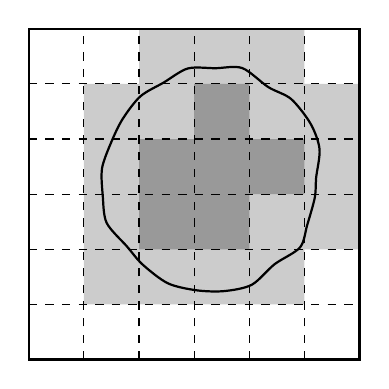
\begin{tikzpicture}[scale=0.7]
                  \pgfmathsetseed{42}

                  \fill[gray!40] (1, 1) -- (1, 5) -- (2, 5) -- (2, 6) -- (5, 6) -- (5, 5) -- (6, 5) -- (6, 2) -- (5, 2) -- (5, 1) -- cycle;
                  \fill[gray!80] (2, 2) -- (2, 4) -- (3, 4) -- (3, 5) -- (4, 5) -- (4, 4) -- (5, 4) -- (5, 3) -- (4, 3) -- (4, 2) -- cycle;

                  \draw[dashed] (0, 0) grid (6, 6);
                  \draw[thick] (0, 0) rectangle (6, 6);

                  \begin{scope}[shift={(3.3, 3.3)}]
                      \path[draw, thick] plot[domain=0:350, smooth cycle] (\x:1.9+0.2*rnd);
                  \end{scope}
              \end{tikzpicture}
              \caption{第一覆盖引理}
          \end{figure}

          \begin{proof}
              对于一个包含 $A$ 的一个矩形 $I$,首先可以定义一个示性函数 $\chi_A$,满足
              \[\chi(x) = \begin{cases}
                      1, & x\in A,    \\
                      0, & x\notin A.
                  \end{cases}\]
              这样 $A$ 的体积就可以表示为 $\nu(A) = \displaystyle\int_I\chi_A$. 因此对于任意的 $\varepsilon >0$,存在 $I$ 的分割 $\pi = \{I_{ij}\}$ 使得\[\left\lvert \sum_{ij}\chi_A(\xi_{ij})\nu(I_{ij}) - \nu(A)\right\rvert < \varepsilon,\enspace \forall \xi_{ij}\in I_{ij}.\]
              根据示性函数的定义,有 \[\sum_{ij}\inf_{\xi_{ij}\in I_{ij}}\chi_A(\xi_{ij})\nu(I_{ij}) = \sum_{I_{ij}\subset A}\nu(I_{ij}),\]
              所以,对于分割 $\pi$ 就有 \[\nu(A) - \varepsilon < \sum_{I_{ij}\subset A}\nu(I_{ij}) \leqslant \nu(A).\]
              同理可以有 \[\sum_{ij}\sup_{\xi_{ij}\in I_{ij}}\chi_A(\xi_{ij})\nu(I_{ij}) = \sum_{I_{ij}\cap A\neq \varnothing}\nu(I_{ij}),\]
              此时就有 \[\nu(A) < \sum_{I_{ij}\cap A\neq \varnothing}\nu(I_{ij}) < \nu(A) + \varepsilon.\]
              这就证明了第一覆盖引理,其中结论中的 $\{I_i\}$ 是 $I_{ij}\subset A$ 的那些 $I_{ij}$,$\{J_j\}$ 是 $I_{ij}\cap A\neq \varnothing$ 的那些 $I_{ij}$.
          \end{proof}

          这个证明的一个副产品就是:这些内部与 $\partial A$ 有非空交集的矩形的体积之和不会超过 $2\varepsilon$,这个结论也不失为一个良好的放缩.

    \item 正交变换. 正交变换就是我们所说的实数域上的等距同构. 对于正交变换 $O\in \mathcal{L}(\mathbf{R}^n)$ 其矩阵表示为 $O_M$,那么就有 $O_MO^\mathrm{T}_M = O_M^\mathrm{T}O_M = I_n$. 正交变换保持向量的模长不变,那么很自然的一点就是,我们可以大胆推断正交变换保持可求体积集合的体积不变,我们下面证明这一点. 首先需要第二覆盖引理.

          \begin{lemma}{第二覆盖引理}{}
              设 $A$ 是 $\mathbf{R}^n$ 中的可求体积的有界集合,则任给 $\varepsilon>0$,存在有限个 $n$ 维球体 $\{B_i\}$ 和 $\{B^j\}$,使得 \[\bigcap_iB_i\subset A \subset \bigcup_jB^j;\enspace \sum_j\nu(B^j) - \varepsilon < \nu(A) < \sum_j\nu(B_i) + \varepsilon,\]
              其中 $\{B_i\}$ 的内部互不相交.
          \end{lemma}

          \begin{figure}[h]
              \centering
              \begin{tikzpicture}[scale=2]
                  \draw (0, 0) grid (2, 2);
                  \foreach \i in {0.5, 1.5}
                      \foreach \j in {0.5, 1.5}
                          \draw[fill=gray!50] (\i, \j) circle (0.5)
                              \foreach \k in {45, 135, 225, 315} {($(\i, \j) + (\k:{sqrt(2)/(sqrt(2)+1)})$) circle ({(sqrt(2)-1)/(2+2*sqrt(2))})};
              \end{tikzpicture}
              \caption{第二覆盖引理}
          \end{figure}

          \begin{proof}
              首先设 $\nu(A)>0$. 我们先取一个矩形 $I = \left[a, b\right]^n$ 使得 $A\subset I$. 将 $I$ 作 $m^n$ 等分,当 $m$ 充分大的时候,完全包含于 $A$ 的小矩形 $\{I_i^1\}$ 的体积之和满足条件 \[\sum_i\nu(I_i^1) > \frac12\nu(A).\]
              矩形 $I_i^1$ 的内接球记为 $B_i^1$,记半径为 $1$ 的 $n$ 维球的体积为 $\omega_n$,根据球体的体积公式或者伸缩变换的结果,我们有 \[\sum_i\nu(B_i^1) = \frac{\omega_n}{2^n}\sum_i\nu(I_i^1) > \frac{\omega_n}{2^{n+1}}\nu(A).\]
              记 \[q = 1 - \frac{\omega_n}{2^{n+1}}\in(0, 1).\]
              由于 $A$ 与 $B_i$ 均可求体积,所以 $A \setminus \bigcup_iB_i^1$ 自然也可求体积(为什么?),因此 \[ 0 < \nu\left(A \setminus \bigcup_iB_i^1\right) < q\nu(A).\]
              我们对 $A\setminus \bigcup\limits_iB_i^1$ 重复上述过程,可以得到包含于 $A\setminus \bigcup\limits_iB_i^1$ 有限个小球体 $\{B_{i'}^2\}$ 使得 \[0 < \nu\left(A\setminus \bigcup_iB_i^1\setminus \bigcup_{i'}B_{i'}^2\right) < q\nu\left(A\setminus \bigcup_iB_i^1\right) < q^2\nu(A).\]
              将这一部分不断重复下去,对于任意的 $\varepsilon > 0$,由于 $q^k\to 0\enspace (k\to \infty)$,所以当 $k$ 充分大的时候,我们就得到内部互不相交的有限个 $n$ 维球体 $\{B_i\}$ 使得 \[0 < \nu\left(A\setminus \bigcup_iB_i\right) < q^k\nu(A) < n^{-n/2}\frac{\varepsilon}{2}.\]
              现在考虑对于 $\overline{A} = A\setminus \bigcup\limits_iB_i$,仍然考虑矩形 $I$ 的 $m^n$ 等分,当 $m$ 充分大的时候,存在着覆盖 $\overline{A}$ 的小矩形 $\{I^j\}$ 使得 \[\sum_j\nu(I^j) < \nu(\overline{A}) + n^{-n/2}\frac{\varepsilon}{2} < n^{-n/2}\varepsilon.\]
              矩形 $I^j$ 的外接球记为 $B_2^j$,那么就有 \[\sum_j\nu(B_2^j) = \frac{\omega_nn^{n/2}}{2^n}\sum_j\nu(I^j) < \frac{\omega_nn^{n/2}}{2^n}n^{-n/2}\varepsilon \leqslant \varepsilon.\]
              这就说明了 $\{B_i, B_2^j\}$ 就是覆盖 $A$ 的 $n$ 维球体,注意到最后一段的证明对于体积为零的情形同样适用,这就完成了第二覆盖引理的证明.
          \end{proof}

          注意,尽管我们通过两个覆盖引理刻画出了可求体积图形的性质,简单定义了一个粗糙的 Jordan ``测度'',但是我们仍然需要谨记:``有限个''这个性质在这里是至关重要的. 更加严格的测度论可以将其推广到 ``可数个'',可以在实分析等课程中学习.

          \begin{theorem}{}{}
              正交变换保持体积不变.
          \end{theorem}

          \begin{proof}
              注意到正交变换将 $n$ 维球映为 $n$ 维球,且球的半径不变,进而其体积不变. 根据第二覆盖引理,正交变换将零体积映为零体积集. 再注意到正交变换将集合的边界点映射为边界点,内点映射为内点,因此将可求体积的集合映为可求体积的集合. 再由覆盖引理及其正交变换保持球体体积变则可知正交变换保持可求体积的集合的体积不变.
          \end{proof}

    \item 一般的线性变换. 设 $\varphi\colon \mathbf{R}^n\to \mathbf{R}^n$ 为线性映射,在 $\mathbf{R}^n$ 的标准基下可以表示为 $n$ 阶方阵,这个方阵仍然记为 $\varphi$. 对于 $\mathbf{R}^n$ 中的可求体积的有界集合 $A$,我们考虑在 $\varphi$ 下的像 $\varphi(A)$. 首先,如果 $\det\varphi = 0$,那么 $\varphi$ 就将 $A$ 压缩成了被某一个超平面包含的集合,这样的集合体积为 $0$,所以我们只考虑 $\det\varphi\neq 0$ 的情况. 这时候 $\varphi\varphi^\mathrm{T}$ 就是正定对称矩阵,根据实谱定理,其可以对角化并且其特征值都大于零,所以其有一个正的平方根 $P$,这样 $\varphi\varphi^\mathrm{T}$ 就可以写为 \[\varphi\varphi^\mathrm{T} = P^2,\]
          其中 $P$ 当然也是正定对称的,且 $\det P = \lvert\det\varphi\rvert$. 这允许我们构造一个正交矩阵 $O = P^{-1}\varphi$,读者可以自行验证它是正交的.

          停下来看一下正定对称矩阵 $P$ 的性质:其对应的线性映射是一个正且自伴的线性映射,我们将其对角化为 $P = O\,\diag(\lambda_1, \lambda_2, \ldots, \lambda_n) O^\mathrm{T}$,其中 $\lambda_i > 0,\enspace 1\leqslant i\leqslant n$,且 $O$ 是一个正交变换. 根据正交变换与伸缩变换的结果,我们得到 \[\nu(P(A)) = (\det P)\nu(A).\]
          结合上面的分析,我们将一个非退化的线性映射 $\varphi$ 分解为一个正交变换与一个正定自伴映射,这就表明如果 $A$ 是可求体积的图形,那么 $\varphi(A) = P(O(A))$ 也是可求体积的,且有 \[\nu(\varphi(A)) = \nu(P(O(A))) = (\det P)\nu(O(A)) = (\det P)\nu(A) = \lvert\det\varphi\rvert \nu(A).\]
\end{enumerate}
简而言之,我们将上述分析总结为下面的定理:

\begin{theorem}{}{}
    对于一般的线性映射 $\varphi\colon \mathbf{R}^n\to \mathbf{R}^n$,与一个可求体积的图形 $A$,其像 $\varphi(A)$ 也是可求体积的,且有 \[\nu(\varphi(A)) = \lvert\det\varphi\rvert \nu(A).\]
\end{theorem}

现在我们要考虑比线性映射更一般的映射,根据``连续可微映射在某一点的局部性质与其在该点的微分的性质相同''这一核心原理,我们可以猜测对于某一点 $p$,如果 $\det J\varphi(p)\neq 0$,对于 $p$ 附近的一个非常小的可求体积的图形 $A$,有 $\nu(\varphi(A)) = \lvert\det J\varphi(p)\rvert \nu(A)$. 对这样的一个个小的面积元进行积分,就是重积分换元法的核心想法. 下面我们给出详细的证明.

设 $D\subset \mathbf{R}^n$ 为开集,$\varphi\colon D\to \mathbf{R}^n$ 为 $C^1$ 映射,根据拟微分中值定理,我们可以知道 $\varphi$ 是一个局部 Lipschitz 映射,也就是任取一个有界闭集 $P\subset D$ 与点 $x, y\in P$,存在 $\rho > 0$ 使得 \[\vert \varphi(x) - \varphi(y)\vert \leqslant \Vert J\varphi(\xi)\Vert \vert x - y\vert \leqslant \rho \vert x - y\vert.\]
所以下面讨论的主题就是如何对可求体积的集合 $A$ 在这样一个局部 Lipschitz 映射下的像 $\varphi(A)$ 的体积进行估计.

\begin{lemma}{}{}
    设 $\varphi\colon\mathbf{R}^n\to \mathbf{R}^n$ 为一个局部 Lipschitz 映射,亦即满足\[\Vert \varphi(x) - \varphi(y)\Vert \leqslant \rho \Vert x - y\Vert,\enspace \forall x, y\in\mathbf{R}^n.\]
    对于一个可求体积的集合 $A\subset \mathbf{R}^n$,如果 $A$ 为零测集,那么 $\varphi(A)$ 也是零测集;如果 $A$ 与 $\varphi(A)$ 都是可求体积的,就有 $\nu(\varphi(A)) \leqslant \rho^n\nu(A)$.
\end{lemma}

\begin{proof}
    设 $A$ 是零测集,则任给 $\varepsilon > 0$,存在至多可数个球体 $B_i = B_{r_i}(x^i)$ 使得 \[A\subset \displaystyle\bigcup_{i\geqslant 1}B_i,\enspace \sum_{i\geqslant 1}\nu(B_i) = \sum_{i\geqslant 1}\omega_n r_i^n < \varepsilon.\]
    由 $\varphi$ 是局部 Lipschitz 的可以得出 $\varphi(B_i) \subset B_{\rho r_i}(\varphi(x^i))$,所以 \[\sum_{i\geqslant 1}\nu(B_{\rho r_i}(\varphi(x^i))) = \sum_{i\geqslant 1}\omega_n (\rho r_i)^n = \rho^n\sum_{i\geqslant 1}\omega_n r_i^n < \rho^n\varepsilon.\]
    这就说明 $\varphi(A)$ 也是零测集.

    设 $A$ 和 $\varphi(A)$ 都是可求体积的,我们使用第二覆盖引理,对于任给的 $\varepsilon > 0$,存在有限个可以覆盖 $A$ 的 $n$ 维球体 $\{B_{r_j}^j\}$ 使得 \[\sum_j\omega_n r_j^n < \nu(A) + \varepsilon.\]
    所以此时 $\varphi(A)$ 被 $\{B_{\rho r_j}^j\}$ 覆盖,因此 \[\nu(\varphi(A))\leqslant \sum_{j}\omega_n (\rho r_j)^n = \rho^n\sum_j\omega_n r_j^n < \rho^n(\nu(A) + \varepsilon).\]
    通过 $\varepsilon$ 的任意性可以得出 $\nu(\varphi(A)) \leqslant \rho^n\nu(A)$.
\end{proof}

事实上,通过反函数定理,如果 $J\varphi$ 处处非退化,那么 $\varphi$ 将内点映射为内点,这就说明如果 $A$ 可求体积,并且 $\overline{A}\subset D$,那么我们对 $\partial \varphi(A)$ 进行放缩:\[\partial \varphi(A) = \overline{\varphi(A)}\setminus \varphi(A)^{\circ} \subset \varphi(\overline{A})\setminus \varphi(A^{\circ}) \subset \varphi(\partial A),\]
由 $A$ 可求体积可以得到 $\partial A$ 是零测集,所以 $\varphi(\partial A)$ 也是零测集,$\partial \varphi(A)$ 仍是零测集,所以 $\varphi(A)$ 就可求体积. 上面的定理只不过给出了 $\varphi(A)$ 体积的一个简单刻画,我们下面将 $\varphi$ 进行线性化并且进行误差估计. 取 $\delta > 0$ 使得 $K = \{x \mid d(x, A) \leqslant \delta\} \subset D$,并记 $C = \max\limits_{x\in K}\Vert J\varphi(x)\Vert$,回忆先前对线性映射与其线性化的映射之间的误差估计,我们可以直接得到下面引理:

\begin{lemma}{}{}
    沿用上面的记号,任给 $\varepsilon >0$,存在 $0<\eta <\delta$,使得当 $x\in A$,$d(x', x)\leqslant \eta$ 时,有 \[\Vert \varphi(x') - \varphi(x) - J\varphi(x)(x' - x)\Vert\leqslant \varepsilon\Vert x' - x\Vert.\]
\end{lemma}

\begin{lemma}{}{}
    沿用上面的记号,则当 $B\subset A$ 可求体积且 $d(B) < \eta$ 时,有 \[\nu(\varphi(B)) \leqslant \left(\lvert \det J\varphi(x)\rvert + O(\varepsilon)\right)\nu(B),\enspace x\in B.\]
\end{lemma}

\begin{proof}
    我们考虑线性变换 $L(y) = \left[J\varphi(x)\right]^{-1}(y - \varphi(x)) + x$ 并记 $F(y) = \varphi(y) - \varphi(x) - J\varphi(x)(x'-x)$,则 \[L\circ\varphi(x') = \left[J\varphi(x)\right]^{-1} F(x') + x'.\]
    于是当 $x', x''\in B_\eta(x)$ 的时候,\[L\circ\varphi(x') - L\circ\varphi(x'') = \left[J\varphi(x)\right]^{-1} (F(x') - F(x'')) + (x' - x'')\leqslant (1 + C\varepsilon)\Vert x' - x''\Vert.\]
    通过 $B\subset B_\eta(x)$ 可以得到 $\nu(L\circ\varphi(B)) \leqslant (1 + C\varepsilon)^n\nu(B)$,所以\[\nu(\varphi(B)) = \frac{\nu(L\circ\varphi(B))}{\lvert \det L\rvert}\leqslant \lvert \det J\varphi(x)\rvert \cdot (1 + C\varepsilon)^n\nu(B) = \left(\lvert \det J\varphi(x)\rvert + O(\varepsilon)\right)\nu(B).\]
    这样就得到了证明.
\end{proof}

\begin{theorem}{重积分换元法}{}
    设 $\varphi\colon D\to \mathbf{R}^n$ 为 $C^1$ 的一个单射,且 $J\varphi$ 处处非退化. 设 $A\subset D$ 为可求体积的集合,$\overline{A}\subset D$,$f$ 在 $\varphi(A)$ 上可积,那么\[\int_{\varphi(A)}f = \int_A f\circ \varphi\lvert \det J\varphi\rvert.\]
    特别地,\[\nu(\varphi(A)) = \int_A \lvert \det J\varphi\rvert.\]
\end{theorem}

\begin{proof}
    根据第一覆盖引理,不妨设 $A$ 为一个矩形,且 $f$ 非负,对于 $A$ 的任意一个分割 $\pi = \{A_{ij}\}$,我们有\[\int_{\varphi(A)}f = \sum_{i, j}\int_{\varphi(A_{ij})}f \leqslant \sum_{i, j}[\sup\limits_{\varphi(A_{ij})}f]\nu(\varphi(A_{ij})).\]
    对于任意的 $\varepsilon$ 当分割充分细,使得 $d(A_{ij})$ 小于某一个 $\eta$ 时,由上述的引理我们知道\[\int_{\varphi(A)}f \leqslant \sum_{i, j}\sup\limits_{A_{i, j}}(f\circ\varphi) \lvert\det J\varphi(\xi_{ij})\rvert \nu(A_{ij}) + O(\varepsilon) = \int_{A}f\circ\varphi\lvert\det J\varphi\rvert + O(\varepsilon).\]
    令 $\varepsilon\to0^+$ 可以得到\[\int_{\varphi(A)}f\leqslant \int_A f\circ\varphi\lvert\det J\varphi\rvert.\]
    根据反函数定理,$\varphi\colon D\to \varphi(D)$ 是可逆的,所以我们对于 $\varphi^{-1}$ 与 $\displaystyle\int_{A}f\circ\varphi\lvert\det J\varphi\rvert$ 进行类似的论证,可以得到 \[\int_{A}f \circ \varphi\lvert \det J\varphi\rvert \leqslant \int_{\varphi(A)}f\circ \varphi\circ\varphi^{-1}\lvert\det J\varphi\rvert \cdot\lvert \det J\varphi^{-1}\rvert  = \int_{\varphi(A)}f.\]
    综上所述,我们有\[\int_{\varphi(A)}f = \int_{A}f\circ\varphi\lvert\det J\varphi\rvert.\]这就完成了证明.
\end{proof}

这样,我们其实可以发现:重积分换元法的核心想法其实是研究\textbf{可求体积的图形在某一个映射下的体积是如何变化的}. 以这个想法为主线,配合\textbf{连续可微映射在某一点的局部性质与其在该点的微分的性质相同}这一核心原理,从线性映射到误差估计,我们就完成了重积分换元法的证明.

\vspace{2ex}
\centerline{\heiti \Large 内容总结}

\vspace{2ex}
\centerline{\heiti \Large 习题}

\vspace{2ex}
{\kaishu }
\begin{flushright}
    \kaishu

\end{flushright}

\centerline{\heiti A组}
\begin{enumerate}
    \item % Schatten 范数 是 范数
          %   设 $A$ 为 $n$ 阶矩阵,定义 $A$ 的 Schatten 范数为 $\Vert A\Vert_s = \left(\sum_{i=1}^n\sigma_i^s\right)^{1/s}$,其中 $\sigma_i$ 为 $A$ 的奇异值. 证明 $\Vert A\Vert_s$ 是一个范数.
\end{enumerate}

\centerline{\heiti B组}
\begin{enumerate}
    \item
\end{enumerate}

\centerline{\heiti C组}
\begin{enumerate}
    \item
\end{enumerate}
